\documentclass[journal]{IEEEtran}
\usepackage{cite}
\usepackage{amsmath}
\usepackage{algorithmic}
\usepackage{array}

% *** SUBFIGURE PACKAGES ***
\ifCLASSOPTIONcompsoc
 \usepackage[caption=false,font=normalsize,labelfont=sf,textfont=sf]{subfig}
\else
 \usepackage[caption=false,font=footnotesize]{subfig}
\fi

% correct bad hyphenation here
\hyphenation{op-tical net-works semi-conduc-tor}


\begin{document}
\title{A survey on vision transformer}

\author{Yuhuan Yang,~\IEEEmembership{MedianBrainGroup,STJU,}}

\maketitle

\begin{abstract}
The abstract goes here.
\end{abstract}

\begin{IEEEkeywords}
IEEE, IEEEtran, journal, \LaTeX, paper, template.
\end{IEEEkeywords}

\IEEEpeerreviewmaketitle

\section{Introduction\cite{w}}
Active contour model, also called snakes, is a framework in computer vision introduced by Michael Kass, Andrew Witkin, and Demetri Terzopoulos\cite{snake} for delineating an object outline from a possibly noisy 2D image. The snakes model is popular in computer vision, and snakes are widely used in applications like object tracking, shape recognition, segmentation, edge detection and stereo matching.

A snake is an energy minimizing, deformable spline influenced by constraint and image forces that pull it towards object contours and internal forces that resist deformation. Snakes may be understood as a special case of the general technique of matching a deformable model to an image by means of energy minimization.\cite{snake} In two dimensions, the active shape model represents a discrete version of this approach, taking advantage of the point distribution model to restrict the shape range to an explicit domain learnt from a training set.

Snakes do not solve the entire problem of finding contours in images, since the method requires knowledge of the desired contour shape beforehand. Rather, they depend on other mechanisms such as interaction with a user, interaction with some higher level image understanding process, or information from image data adjacent in time or space.

\section{Snakes model}
The snake model was first introduced in 1988 by Kass\cite{snake}. The basic idea of this paper is define snake model as a \textit{controlled continuity}\cite{s18} spline under the influence of image forces and external constraint forces. Representing the position of a snake parametrically by $\mathbf{v}(s)=(x(s),y(s))$, the energy function of snake model can be written as:
\begin{equation}\begin{aligned}
E_{\text{snake}}=&\int_0^1 E_{\text{snake}}(\mathbf{v}(s))ds\\
=&\int_0^1 E_{\text{int}}(\mathbf{v}(s))+E_{\text{image}}(\mathbf{v}(s))\\
&+E_{\text{con}}(\mathbf{v}(s))ds,\label{eq1}
\end{aligned}\end{equation}
where $E_{\text{int}}$ represents the internal energy of the spline due to bending, $E_{\text{image}}$ gives rise to the image forces, and $E_{\text{con}}$ represents the external constraint forces. In the following section, we introduce all of the three energy in detail.
\subsection{Internal Energy}
The internal spline energy can be written as:
\begin{equation}\begin{aligned}
E_{\text{int}}=(\alpha(s)\|\mathbf{v}'(s)\|^2+\beta(s)\|\mathbf{v}''(s)\|^2).
\end{aligned}\end{equation}
The internal part of spline energy is composed of a first-order term comtrolled by $\alpha(s)$ and a second-order term controlled by $\beta(s)$. The first-order term makes the snake act like a membrane, and the second-order term makes it act like a thing plate. By adjusting the weight of $\alpha(s)$ and $\beta(s)$, we can control the relative importance of the membrane and thin-plate terms.
\subsection{Detailed minimizing procedure}
When $\alpha(s)$ and $\beta(s)$ are constants, minimizing the energy function\ref{eq1} gives rise to the following two independent Euler equations:
\begin{equation}\begin{aligned}
\alpha x''+\beta x''''+\frac{\partial E_{\text{ext}}}{\partial x}=0\\
\alpha y''+\beta y''''+\frac{\partial E_{\text{ext}}}{\partial x}=0
\end{aligned}\end{equation} 
When $\alpha(s)$ and $\beta(s)$ are not constant, is's simpler to go directly to a discrete formulation as:
\begin{equation}\begin{aligned}
E_{\text{snake}}=\sum_{i=1}^n E_{\text{int}}(i)+E_{\text{ext}}(i)
\end{aligned}\end{equation}
Approximating the derivatives with finite differences and converting to vector notation with $\mathbf{v}_i=(x_i,y_i)=(x(ih),y(ih))$, we have:
\begin{equation}\begin{aligned}
E_{\text{int}}(i)=&\alpha_i |\mathbf{v}_i-\mathbf{v}_{i-1}|^2/2h^2\\
&+\beta_i|\mathbf{v}_{i-1}-2\mathbf{v}_i+\mathbf{v}_{i+1}|^2/2h^4.
\end{aligned}\end{equation}
Let $f_x(i)=\frac{\partial E_{\text{ext}}}{\partial x_i}$ and $f_y(i)=\frac{\partial E_{\text{ext}}}{\partial y_i}$, the corresponding Euler equation becomes:
\begin{equation}\begin{aligned}
    \alpha_{i}\left(\mathbf{v}_{i}-\mathbf{v}_{i-1}\right)&- \alpha_{i+1}\left(\mathbf{v}_{i+1}-\mathbf{v}_{i}\right) \\
    &+\beta_{i-1}\left[\mathbf{v}_{i-2}-2 \mathbf{v}_{i-1}+\mathbf{v}_{i}\right] \\
    &-2 \beta_{i}\left[\mathbf{v}_{i-1}-2 \mathbf{v}_{i}+\mathbf{v}_{i+1}\right] \\
    &+\beta_{i+1}\left[\mathbf{v}_{i}-2 \mathbf{v}_{i+1}+\mathbf{v}_{i+2}\right] \\
    &+\left(f_{x}(i), f_{y}(i)\right)=0
\end{aligned}\end{equation}
The above Euler equations can be written in matrix form as:
\begin{equation}\begin{aligned}
\mathbf{Ax+f_x(x,y)}=0\\
\mathbf{Ay+f_y(x,y)}=0 \label{eq2}
\end{aligned}\end{equation}
where $A$ is a pentadiagonal banded matrix.

The equation \ref{eq2} can be rewrite in the format of time derivative as:
\begin{equation}\begin{aligned}
  \mathbf{Ax_t+f_x(x_{t-1},y_{t-1})}=-\gamma(\mathbf{x_t-x_{t-1}})\\
  \mathbf{Ay_t+f_y(x_{t-1},y_{t-1})}=-\gamma(\mathbf{y_t-y_{t-1}}) \label{eq3}
\end{aligned}\end{equation}
and the equation \ref{eq3} can be soved by matrix inversion:
\begin{equation}\begin{aligned}
\mathbf{x_t}=(\mathbf{A}+\gamma\mathbf{I})^{-1}(\mathbf{x_{t-1}-f_x(x_{t-1},y_{t-1})})\\
\mathbf{y_t}=(\mathbf{A}+\gamma\mathbf{I})^{-1}(\mathbf{y_{t-1}-f_y(x_{t-1},y_{t-1})})\label{eq5}
\end{aligned}\end{equation}

\section{Introduction}

\IEEEPARstart{T}{his} demo file is intended to serve as a ``starter file''
for IEEE journal papers produced under \LaTeX\ using
IEEEtran.cls version 1.8b and later.

\subsection{Subsection Heading Here}
Subsection text here.

\subsubsection{Subsubsection Heading Here}
Subsubsection text here.


%\begin{figure}[!t]
%\centering
%\includegraphics[width=2.5in]{myfigure}
%\caption{Simulation results for the network.}
%\label{fig_sim}
%\end{figure}

%\begin{figure*}[!t]
%\centering
%\subfloat[Case I]{\includegraphics[width=2.5in]{box}%
%\label{fig_first_case}}
%\hfil
%\subfloat[Case II]{\includegraphics[width=2.5in]{box}%
%\label{fig_second_case}}
%\caption{Simulation results for the network.}
%\label{fig_sim}
%\end{figure*}
%

\begin{table}[!t]
%% increase table row spacing, adjust to taste
\renewcommand{\arraystretch}{1.3}
% if using array.sty, it might be a good idea to tweak the value of
% \extrarowheight as needed to properly center the text within the cells
\caption{An Example of a Table}
\label{table_example}
\centering
%% Some packages, such as MDW tools, offer better commands for making tables
%% than the plain LaTeX2e tabular which is used here.
\begin{tabular}{|c||c|}
\hline
One & Two\\
\hline
Three & Four\\
\hline
\end{tabular}
\end{table}
\subsection{Image forces}
In order to make snakes useful for early vision we need energy functions that attract them to salient features in image. Generally, the image energy functions should attract a snake to lines, edges, and terminations. The total image energy can be expressed as a weighted combination of the three terms:
\begin{equation}\begin{aligned}
E_{\text{image}}=w_{\text{line}}E_{\text{line}}+w_{\text{edge}}E_{\text{edge}}+w_{\text{term}}E_{\text{term}}.
\end{aligned}\end{equation}
Now we introduce some simple but useful image energy terms.
\subsubsection{Line function}
The simplest useful image function is the image intensity it self. If we set
\begin{equation}\begin{aligned}
E_{\text{line}}=I(x,y),
\end{aligned}\end{equation}
then, depending on the sign of $w_{\text{line}}$, the snake will be attracted either to light lines or dark lines.
\subsubsection{Edge function}
Finding edges in an image can also be done with a very simple energy function by just setting:
\begin{equation}\begin{aligned}
E_{\text{edge}}=-|\nabla I(x,y)|^2.\label{eq4}
\end{aligned}\end{equation}
With this function, the snake will be attracted to contours with large image gradients.
\subsubsection{Scale space}
One can allow the snake to come to equilibrium on a very blurry energy function and then slowly reduce the blurring. The result is minimization by scale-continuation.\cite{s20},\cite{s21} Thus, a new format of edge energy function is developed as:
\begin{equation}\begin{aligned}
E_{\text{line}}=-(G_\sigma * \nabla^2I)^2,
\end{aligned}\end{equation}
where $G_\sigma$ is a Gaussian of standard deviation $\sigma$.
\subsubsection{Termination function}
In order to find terminations of line segments and corners, we use the curvature of level lines in a slightly smoothed image. Let $C(x,y)=G_\sigma(x,y)*I(x,y)$ be a slightly smoothed version of the image, let $\theta=\tan^{-1}{(C_y/C_x)}$ be the gradient angle and let $\mathbf{n}=(\cos \theta,\sin\theta),\mathbf{n}_\perp=(-\sin\theta,\cos\theta)$, the curvature of level contours in $C(x,y)$ can be written as:
\begin{equation}\begin{aligned}
    E_{\mathrm{tem}} &=\frac{\partial \theta}{\partial \mathbf{n}_{\perp}} \\
    &=\frac{\partial^{2} C / \partial \mathbf{n}_{\perp}^{2}}{\partial C / \partial \mathbf{n}} \\
    &=\frac{C_{y y} C_{x}^{2}-2 C_{x y} C_{x} C_{y}+C_{x x} C_{y}^{2}}{\left(C_{x}^{2}+C_{y}^{2}\right)^{3 / 2}}
\end{aligned}\end{equation}

\section{Snake with bolloon force}
The snake model achieves great success in image segmentation and recognition, however, it has some weaknesses that should not be ignored. The original sname, when note closed enough to contours, is not attracted by them and straightens to a line. Thus, in 1989, Cohen\cite{balloon} pointed out the weakness of original snake model, and came up with a new format of external force which makes the curve behave like a balloon. The initial curve need no longer to be close to the solution to converge, it can inflate by an additional force, pass over weak edges and be stopped only if the edge is strong.

\subsection{The Instability of original smake model}
The most used format of external force for snake model is the edge function defined as equation \ref{eq4}. We define the potential of shape as $\int_0^1 P(v(s))ds$ where:
\begin{equation}\begin{aligned}
P(v)=E_{\text{edge}}=-|\nabla I(v)|^2.\notag
\end{aligned}\end{equation}
The equation \ref{eq5} can be rewrite as:
\begin{equation}\begin{aligned}
(I+\gamma A)v_t=(v_{t-1}+\gamma F(v_{t-1})).\label{eq6}
\end{aligned}\end{equation}
where $F=-\nabla P$ is the external force.

However, even though the initial guess can be close to an edge, instabilities can occur due to the discretization of the evolution problem. We can see from equation \ref{eq6} that, the position at time $t, v_t$ is obtained after moving $v_{t-1}$ alone vector $\gamma F(v_{t-1})$ and then solving the system. This leads to the following remarks:
\paragraph{Time Discretization} If $\gamma F(v_{t-1})$ is too large the point $v_{t-1}$ can be moved too far across the desired minimum and never come back. So the curve can pass through the dege and then make large oscillations without reaching equilibrium, or stabilize to a different minimum.

This problem can be solved to choose time step $\gamma$ small enough such that move $\gamma F(v_{t-1})$ is never too large. However, only very few high gradient points will attract the curve and small $F$ will not affect much the curve, since they are too small compared with the internal forces. Thus, instead of acting on the time step, bolloon model modify the force by normalizing it, taking $F=-k\frac{\partial P}{\|\partial P\|}$ where $k$ is mannually chosen that $k\gamma$ is on the order of the pixel size.

\paragraph{Space Discretization}The force F is known only on a discrete grid corresponding to the image, and therefore, there can be a zero-crossing without any zero in the grid. This problem is simply solved by bilinear interpolation of F at a noninteger positions.

\subsection{The bollon force}
To make the snake find its way, an initial guess of the contour has to be provided manually. This has many consequences for the evolution of the curve:
\begin{itemize}
  \item If the curve is not close enough to an edge, it is not attracted by it.
  \item If the curve is not submitted by any forces, it shrinks on itself.
\end{itemize}
To fix this problem, from an initial oriented curve, a new force is added as a pressure pushing outside as if we introduced air inside. The modified format of F now becomes:
\begin{equation}\begin{aligned}
F=k_1\mathbf{n}(s)-k\frac{\nabla P}{\|\nabla P\|}
\end{aligned}\end{equation}
where $\mathbf{n}(s)$ is the normal unitary vector to the curve at point $v(s)$ and $k_1$ is the amplitude of this force. If we
change the sign of $k_1$ or the orientation of the curve, it will
have an effect of deflation instead of inflation. $k_1$, and $k$ are chosen such that they are of the same order, which is
smaller than a pixel size, and $k$ is slightly larger than $k_1$ so an edge point can stop the inflation force. The curve then
expands and it is attracted and stopped by edges as before. But since there is a pressure force, if the edge is too
weak the curve can pass through this edge if it is a singularity with regard to the rest of the curve being inflated.
This means that it tends to create a tangent discontinuity
at this point. The smoothing effect with the help of the
inflation force then removes the discontinuity and the
curve passes through the edge.

\section{Active contour without edges}
However, the snake models metioned above all rely on the edge-function, and depends on the image gradient $\nabla I$, to stop the curve evolution, these models can detect only objects with edges defined by gradient. In practice, the discrete gradients are bounded and then the stopping function is never zero on the edges, and the curve may pass through the boundary. What's more, if the image is very noisy, then  the isotropic smoothing Gaussian has to be strong, which will smooth the edges too.

To fix this problem, Chan\cite{ne} propose a different active contour model, without a stopping edge-function, i.e. a model which is not based on the gradient of the image for the stopping process. The stopping term is based on Mumford–Shah segmentation techniques \cite{ne18}. In this way, we obtain a model which can detect contours both with or without gradient, for instance objects with very smooth boundaries or even with discontinuous boundaries.

\subsection{Model description}
Define the evolving curve $C$ in $\Omega$, as the boundary of an open subset $\omega$ of $\Omega$(i.e. $\omega\in\Omega, C=\partial\omega$). Thus, $inside(C)$ denootes the region $\omega$ and $outside(C)$ denotes the region $\Omega\backslash\bar{\omega}$.

The model introduce the energy function $F(c_1,c_2,C)$ defined bt:
\begin{equation}\begin{aligned}
    F\left(c_{1}, c_{2}, C\right)&= \mu \cdot \text { Length }(C)+\nu \cdot \operatorname{Area}(i n \operatorname{side}(C)) \\
    &+\lambda_{1} \int_{\text {inside }(C)}\left|u_{0}(x, y)-c_{1}\right|^{2} d x d y \\
    &+\lambda_{2} \int_{\text {outside }(C)}\left|u_{0}(x, y)-c_{2}\right|^{2} d x d y,
\end{aligned}\end{equation}
where $\mu\geq 0, \nu\geq 0, \lambda_1,\lambda_2>0$ are fixed parameters. The following introdution fix $\lambda_1=\lambda_2=1$ and $\nu=0$.
\subsection{Level set formulation of the model}
In the level set method\cite{ne19}, $C\in\Omega$ is represented by the zero level set of a Lipschitz function $\phi:\Omega\to\mathcal{R}$ such that:
\begin{equation}
  \left\{\begin{array}{l}
  C=\partial \omega=\{(x, y) \in \Omega: \phi(x, y)=0\} \\
  \text { inside }(C)=\omega=\{(x, y) \in \Omega: \phi(x, y)>0\} \\
  \text { outside }(C)=\Omega \backslash \bar{\omega}=\{(x, y) \in \Omega: \phi(x, y)<0\}
  \end{array}\right.
\end{equation}
Using the Heaviside function $H$ and the one-dimensional Dirac measure $\delta_0$ defined respectively by
\begin{equation}
  H(z)=\left\{\begin{array}{ll}
  1, & \text { if } z \geq 0 \\
  0, & \text { if } z<0,
  \end{array} \quad \delta_{0}(z)=\frac{d}{d z} H(z)\right.
\end{equation}
the term of energy $F$ can be expressed in the following way:
\begin{equation}
  \begin{aligned}
  \text { Length }\{\phi=0\} &=\int_{\Omega}|\nabla H(\phi(x, y))| d x d y \\
  &=\int_{\Omega} \delta_{0}(\phi(x, y))|\nabla \phi(x, y)| d x d y, \\
  \text { Area }\{\phi \geq 0\} &=\int_{\Omega} H(\phi(x, y)) d x d y,
  \end{aligned}
\end{equation}
and
\begin{equation}
  \begin{aligned}
  &\int_{\phi>0}\left|u_{0}(x, y)-c_{1}\right|^{2} d x d y \\
  &\quad=\int_{\Omega}\left|u_{0}(x, y)-c_{1}\right|^{2} H(\phi(x, y)) d x d y \\
  &\int_{\phi<0}\left|u_{0}(x, y)-c_{2}\right|^{2} d x d y \\
  &\quad=\int_{\Omega}\left|u_{0}(x, y)-c_{2}\right|^{2}(1-H(\phi(x, y))) d x d y .
  \end{aligned}
\end{equation}
Then, the energy $F(c_1,c_2,\phi)$ can be written as:
\begin{equation}
  \begin{aligned}
  F\left(c_{1},\right.&\left.c_{2}, \phi\right) \\
  =& \mu \int_{\Omega} \delta(\phi(x, y))|\nabla \phi(x, y)| d x d y \\
  &+\nu \int_{\Omega} H(\phi(x, y)) d x d y \\
  &+\lambda_{1} \int_{\Omega}\left|u_{0}(x, y)-c_{1}\right|^{2} H(\phi(x, y)) d x d y \\
  &+\lambda_{2} \int_{\Omega}\left|u_{0}(x, y)-c_{2}\right|^{2}(1-H(\phi(x, y))) d x d y
  \end{aligned}
\end{equation}
Keeping $\phi$ fixed and minimizing the energy $F(c_1,c_2,\phi)$ with respect to the constants $c_1$ and $c_2$, it is easy to express these constants function of $\phi$ by:
\begin{equation}
  c_{1}(\phi)=\frac{\int_{\Omega} u_{0}(x, y) H(\phi(x, y)) d x d y}{\int_{\Omega} H(\phi(x, y)) d x d y}
\end{equation} 
If $\int_\Omega H(\phi(x,y))d x d y >0$ then:
\begin{equation}
  c_{2}(\phi)=\frac{\int_{\Omega} u_{0}(x, y)(1-H(\phi(x, y))) d x d y}{\int_{\Omega}(1-H(\phi(x, y))) d x d y}
\end{equation}
IF $\int_\Omega(1-H(\phi(x,y)))d x d y>0$ (i.e. if the curve has a nonempty exterior in $\Omega$). For the corresponding ``degenerate'' cases, there are no constrains on the value of $c_1$ and $c_2$. Then, $c_1$ and $c_2$ are in fact given by:
\begin{equation}
  \left\{\begin{array}{l}
  c_{1}(\phi)=\operatorname{average}\left(u_{0}\right) \text { in }\{\phi \geq 0\} \\
  c_{2}(\phi)=\operatorname{average}\left(u_{0}\right) \text { in }\{\phi<0\}
  \end{array}\right.
\end{equation}

\subsection{Numerical approximation}
In order to compute the associated Euler-Langrange equation for the unknown function $\phi$, we consider slightly regularized versions of the functions $H$ and $\delta_0$, denotes as $H_\epsilon$ and $\delta_\epsilon$ as $\epsilon\to 0$. Let $H_\epsilon$ beany $C^2(\hat{\Omega})$ regularization of $H$ and $\delta_\epsilon=H_\epsilon'$, The associated regulaized energy function can be expressed as $F_\epsilon$.

Keeping $c_1$ and $c_2$ fixed, and minimizing $F_\epsilon$ with respect to $\phi$, we deduce the associated Euler-Langrange equattion for $\phi$. Parameterizing the descent direction by an artificial time $t\geq 0$, the equation in $\phi(t,x,y)$(with $\phi(0,x,y)=\phi_0(x,y)$ defining the initial contour) is:
\begin{equation}\begin{aligned}
    \frac{\partial \phi}{\partial t}=\delta_{\varepsilon}(\phi) &\left[\mu \operatorname{div}\left(\frac{\nabla \phi}{|\nabla \phi|}\right)-\nu-\lambda_{1}\left(u_{0}-c_{1}\right)^{2}\right.\\
    &\left.+\lambda_{2}\left(u_{0}-c_{2}\right)^{2}\right]=0 \text { in }(0, \infty) \times \Omega, \\
    & \phi(0, x, y)=\phi_{0}(x, y) \text { in } \Omega, \\
    & \frac{\delta_{\varepsilon}(\phi)}{|\nabla \phi|} \frac{\partial \phi}{\partial \vec{n}}=0 \text { on } \partial \Omega.
\end{aligned}\end{equation}
where $\vec{n}$ denotes the exterior normal to the boundary $\partial\Omega$, and $\partial\phi/\partial\vec{n}$ denotes the normal derivative of $\phi$ at the boundary.

And two possible regularization of $H$ by $C^2(\bar{\Omega})$ functions are:
\begin{equation}
  H_{1, \varepsilon}(z)=\left\{\begin{array}{l}
  1 \text { if } z>\varepsilon \\
  0 \text { if } z<-\varepsilon \\
  \frac{1}{2}\left[1+\frac{z}{\varepsilon}+\frac{1}{\pi} \sin \left(\frac{\pi z}{\varepsilon}\right)\right] \text { if }|z| \leq \varepsilon
  \end{array}\right.
\end{equation}
\begin{equation}
  H_{2, \varepsilon}(z)=\frac{1}{2}\left(1+\frac{2}{\pi} \arctan \left(\frac{z}{\varepsilon}\right)\right) .
\end{equation}

\section{Deep snake models}
In recent years, with the increasing popularity of deep learning, the combination of serpentine model and deep neural network has also produced impressive results.
\subsection{Level set regression}
In deep learning, image segmentation is often considered as a pixel-wise classification task. However, with the definition of level set, it's easily transformed into a level-set regression task, which facilitates learning. \cite{gsnake} proposes a level set function regression network supervised by the segmentation ground truth and geodesic active contours. With the help of geodesic active contours, the segmentation contour, embedded in the level set function, can be globally driven towards the image boundary to obtain lower energy, and the geodesic constraint can lead the segmentation result to have fewer outliers. 

\subsubsection{Method}
Firstly, the author define an image edge indicator function $g_I$ as :
\begin{equation}
  g_{I}=\frac{1}{1+\left|\nabla G_{\sigma} * I\right|^{2}}
\end{equation}
and the energy function $E(\phi)$ is defined by:
\begin{equation}
  E(\phi)=\int_{\Omega} g_{I} \delta_{\epsilon}(\phi)|\nabla \phi| d x
\end{equation}
where:
\begin{equation}
  \delta_{\epsilon}=\frac{\epsilon}{\pi\left(\phi^{2}+\epsilon^{2}\right)}
\end{equation}
The network architecture for this method is designed as a multi-head structure, with one branch predicting the probability map for final segmentation class, and supervised by ground truth using dice loss:
\begin{equation}
  L_{\text {Dice }}=1-\frac{2 \sum_{i=1}^{N} s_{i} g_{i}}{\sum_{i=1}^{N} s_{i}^{2}+\sum_{i=1}^{N} g_{i}^{2}}
\end{equation}
and the second branch optimized by minimizing the energy function $E(\phi)$, the last branch supervised by the level set. The whole pipeline is shown in Fig. \ref{fig:gseg}.

\begin{figure}[htp] 
	\centering
	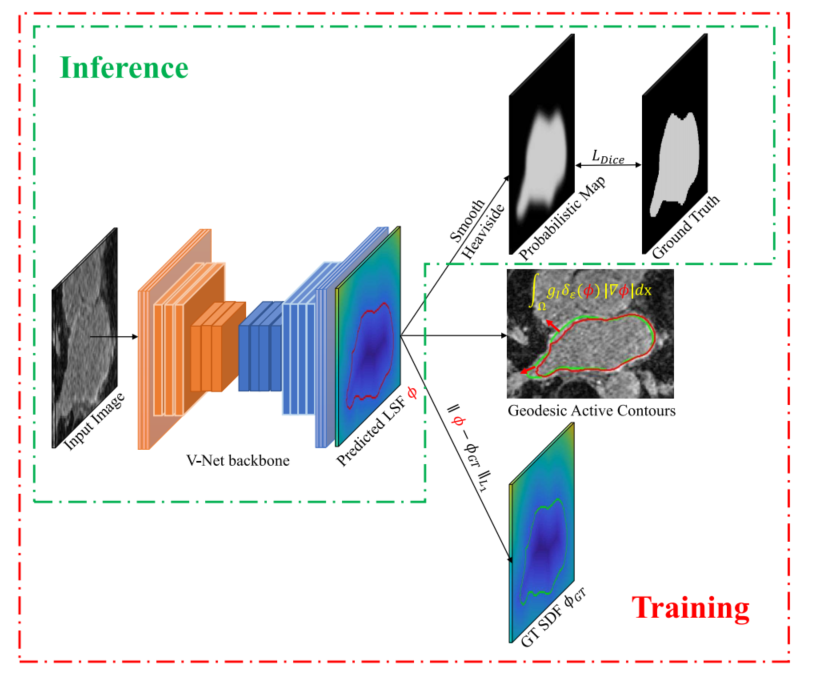
\includegraphics[width=1\linewidth]{../imgs/gseg.png}%
	%\vspace{-1em}
	\caption{The pipeline of the training and inference structure in \cite{gsnake}}
	\label{fig:gseg}
\end{figure}

\subsection{Feature engineering}
Feature engineering is another kind of way to combine deep learning and traditional methods. In the setting of feature engineering, neural networks don't give out the final result, but some intermediant representation or parameter for the white-box model. Compared with fully deep method, feature engineering give more explainity to the model. And compared with traditional method, it can gain more accuracy and reduce the cost of fine tuning parameter. \cite{evlove} proposes a network which absorb the idea of feature engineering. The whole pipeline is shown in Fig. \ref{fig:evolve}

\begin{figure*}[htp] 
	\centering
	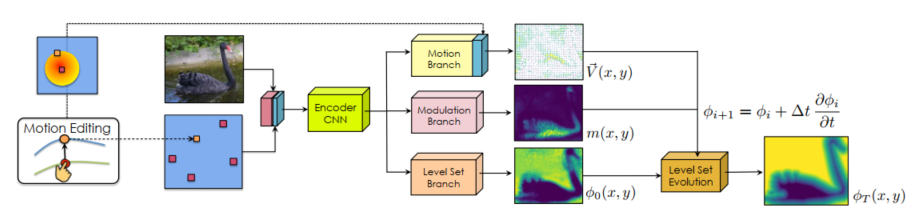
\includegraphics[width=1\linewidth]{../imgs/evolve.png}%
	%\vspace{-1em}
	\caption{The pipeline of the training and inference structure in \cite{evlove}}
	\label{fig:evolve}
\end{figure*}

The evolve function defined in this article is:
\begin{equation}
  \frac{\partial \phi(s, t)}{\partial t}=V \vec{N}
\end{equation}
where $\phi$ is the level set, $V$ is the velocity of the evolution. The network directly predicts $V$ under the supervise of ground truth level-set generated by mask. The direction can be formed as:
\begin{equation}
  \vec{U}_{\mathrm{gt}}(x, y)=-\frac{\nabla \phi_{D T}(x, y)}{\left|\nabla \phi_{D T}(x, y)\right|}
\end{equation}
and since we want the predicted motion of the curve is similar to the ground truth, we maximize the cosin similarity of predicted vector and the gradient:
\begin{equation}
  \left[\frac{\partial \phi_{i}}{\partial t}\right]_{\text {motion }}=-\left\langle\vec{V}_{\theta}, \nabla \phi_{i}\right\rangle.
\end{equation}
Two prevent the curve from dramatic change, two reqularization term has also be added, one is curvature, in the form of:
\begin{equation}
  \begin{aligned}
  \left[\frac{\partial \phi_{i}}{\partial t}\right]_{\text {curvature }} &=m_{\theta} \kappa\left|\nabla \phi_{i}\right| \\
  &=m_{\theta}\left|\nabla \phi_{i}\right| \operatorname{div}\left(\frac{\nabla \phi_{i}}{\left|\nabla \phi_{i}\right|}\right) 
  \end{aligned}
\end{equation}
and another is distance reqularization term which restrict the behavior of evolution by:
\begin{equation}
  \left[\frac{\partial \phi_{i}}{\partial t}\right]_{\mathrm{reg}}=\operatorname{div}\left(p^{\prime}\left(\left|\nabla \phi_{i}\right|\right) \frac{\nabla \phi_{i}}{\left|\nabla \phi_{i}\right|}\right).
\end{equation}
Finally, we combine all three terms from the prediction of internet and get the evolution rule for level-set:
\begin{equation}
  \begin{aligned}
  \frac{\partial \phi_{i}}{\partial t}=&-\left\langle\vec{V}_{\theta}, \nabla \phi_{i}\right\rangle+\lambda \cdot m_{\theta}\left|\nabla \phi_{i}\right| \operatorname{div}\left(\frac{\nabla \phi_{i}}{\left|\nabla \phi_{i}\right|}\right) \\
  &+\mu \cdot \operatorname{div}\left(p^{\prime}\left(\left|\nabla \phi_{i}\right|\right) \frac{\nabla \phi_{i}}{\left|\nabla \phi_{i}\right|}\right)
  \end{aligned}
\end{equation}
\section{Conclusion}
The conclusion goes here.\cite{han2020survey}

% Can use something like this to put references on a page
% by themselves when using endfloat and the captionsoff option.
\ifCLASSOPTIONcaptionsoff
  \newpage
\fi

% references section
\bibliographystyle{IEEEtran}
\bibliography{IEEEabrv,../bib/paper}

\end{document}


